%
% Copyright 2018 Joel Feldman, Andrew Rechnitzer and Elyse Yeager.
% This work is licensed under a Creative Commons Attribution-NonCommercial-ShareAlike 4.0 International License.
% https://creativecommons.org/licenses/by-nc-sa/4.0/
%
\questionheader{ex:s1.3}

%%%%%%%%%%%%%%%%%%
\subsection*{\Conceptual}
%%%%%%%%%%%%%%%%%%

\begin{question}[2016Q2]
Suppose that $f(x)$ is a function and $F(x) = e^{(x^2-3)} + 1$ is an antiderivative of $f(x)$. Evaluate the definite integral $\displaystyle\int_1^{\sqrt5} f(x)\,\dee{x}$.
\end{question}

%\begin{hint}
%\end{hint}

\begin{answer}
$e^2-e^{-2}$
\end{answer}

\begin{solution}
The Fundamental Theorem of Calculus Part 2 (Theorem \eref{CLP101}{thm:INTfundthmofcalc}
 in the CLP-2 text) tells us that
\begin{align*}
\int_1^{\sqrt5} f(x)\,\dee{x} &= F(\sqrt5) - F(1) \\
&= \big( e^{(\sqrt5^2-3)} + 1 \big) - \big( e^{(1^2-3)} + 1 \big) \\
&= e^{5-3} - e^{1-3} = e^2-e^{-2}
\end{align*}
\end{solution}
%%%%%%%%%%%%%%%%%%%

\begin{question}[M105 2015A]
For the function $f(x) = x^3 -\sin 2x$, find its antiderivative $F(x)$ that
satisfies $F(0)=1$.
\end{question}

\begin{hint}
First find the general antiderivative by guessing and checking.
\end{hint}

\begin{answer}
$F(x) = \dfrac{x^4}{4}+\dfrac{1}{2}\cos 2x+\dfrac{1}{2}$.
\end{answer}

\begin{solution}
First, let's find a general antiderivative of $x^3-\sin(2x)$.
\begin{itemize}
\item One function with derivative $x^3$ is $\dfrac{x^4}{4}$.
\item  To find an antiderivative of $\sin(2x)$, we might first guess $\cos(2x)$; checking, we see $\diff{}{x}\{\cos(2x)\}=-2\sin(2x)$. So, we only need to multiply by $-\dfrac{1}{2}$: $\displaystyle\diff{}{x}\left\{-\dfrac{1}{2}\cos 2x\right\}=\sin(2x)$.
\end{itemize}
So, the general antiderivative
of $f(x)$ is $\dfrac{x^4}{4}+\dfrac{1}{2}\cos 2x+C$. To satisfy $F(0)=1$,
we need\footnote{The symbol
$\iff$ is read ``if and only if''. This is used in mathematics to
express the logical equivalence of two statements. To be more precise,
the statement $P \iff Q$ tells us that $P$ is true whenever $Q$ is true
and $Q$ is true whenever $P$ is true.}
\begin{align*}
\Big[\frac{x^4}{4}+\frac{1}{2}\cos 2x+C\Big]_{x=0}=1
\iff \frac{1}{2} + C = 1
\iff C=\frac{1}{2}
\end{align*}
So $F(x) = \dfrac{x^4}{4}+\dfrac{1}{2}\cos 2x+\dfrac{1}{2}$.
\end{solution}
%%%%%%%%%%%%%%%%%%%

\begin{Mquestion}[2014D]
Decide whether each of the following statements is true or false.
Provide a brief justification.

\begin{enumerate}[(a)]
\item
If $f(x)$ is continuous on $[1, \pi]$ and differentiable on $(1,\pi)$, then
           $\displaystyle\int_1^\pi f'(x)\,\dee{x} = f(\pi)-f(1)$.
\item
 $\displaystyle\int_{-1}^1 \frac{1}{x^2}\,\dee{x} = 0$.

\item
If $f$ is continuous on $[a, b]$ then
           $\displaystyle\int_a^b xf(x)\,\dee{x} = x\int_a^b f(x)\,\dee{x} $.

\end{enumerate}
\end{Mquestion}

\begin{hint}
Be careful. Two of these make no sense at all.
\end{hint}

\begin{answer}
(a) True
\qquad (b) False
\qquad (c) False, unless $\int_a^b f(x)\,\dee{x}=\int_a^b xf(x)\,\dee{x} = 0$.
\end{answer}

\begin{solution} (a)
This is true, by part 2 of the Fundamental Theorem of Calculus,
Thereom \eref{CLP101}{thm:INTfundthmofcalc} in the CLP-2 text
with $G(x)=f(x)$ and $f(x)$ replaced by $f'(x)$.


\noindent (b)
This is not only false, but it makes no sense at all. The integrand
is strictly positive so the integral has to be strictly positive. In fact it's
$+\infty$. The Fundamental Theorem of Calculus does not apply because the integrand has an infinite discontinuity at $x=0$.

\begin{center}
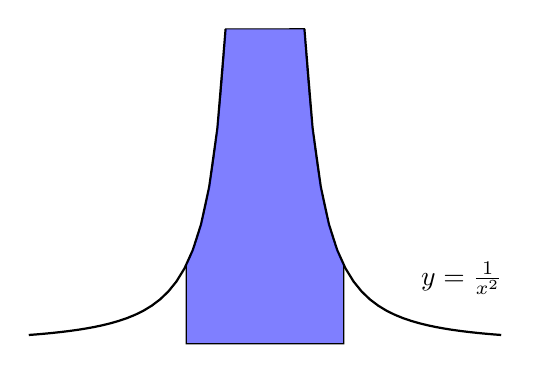
\begin{tikzpicture}
\YEaaxis{3.5}{3.5}{1}{4.25}
\YExcoord{-1}{-1}
\YExcoord{1}{1}
\draw[thick] plot[domain=-3:-0.5](\x,{1/(\x*\x)});
\draw[thick] plot[domain=.5:3](\x,{1/(\x*\x)});
\draw (2.5,.5) node[above] {$y=\frac{1}{x^2}$};
\draw[fill=blue, fill opacity=0.5] plot[domain=-1:-0.5](\x,{1/(\x*\x)})--(.5,4)--
plot[domain=.5:1](\x,{1/(\x*\x)})--(1,0)--(-1,0)--cycle;
\end{tikzpicture}
\end{center}
\noindent (c)
This is not only false, but it makes no sense at all, unless
$\int_a^b f(x)\,\dee{x}=\int_a^b xf(x)\,\dee{x} = 0$. The left hand
side is a number. The right hand side is a number times $x$.

\[\underbrace{\int_a^b xf(x)\ \dee{x}}_{\mathrm{area}} \qquad\mbox{vs}\qquad \underbrace{x}_{\mathrm{variable}}\cdot\underbrace{\int_a^bf(x)\ \dee{x}}_{\mathrm{area}}\]

For example,
if $a=0$, $b=1$ and $f(x) = 1$, then the left hand side is
$\int_0^1 x\,\dee{x} = \frac{1}{2}$ and the right hand side is
$x\int_0^1 \dee{x}=x$.
\end{solution}
%%%%%%%%%%%%%%%%%%%

\begin{Mquestion} True or false: an antiderivative of $\dfrac{1}{x^2}$ is $\log (x^2)$ (where by $\log x$ we mean
logarithm base $e$).
\end{Mquestion}
\begin{hint}
Check by differentiating.
\end{hint}
\begin{answer} false
\end{answer}
\begin{solution}
This is a tempting thought:
\begin{align*}
\int \frac{1}{x}\ \dee{x}&=\log|x|+C
\intertext{ so perhaps similarly }
\int \frac{1}{x^2}\ \dee{x}&\stackrel{?}{=}\log|x^2|+C=\log(x^2)+C
\intertext{ We check by differentiating:}
\diff{}{x}\{\log(x^2)\} &= \diff{}{x}\{2\log x\}=\frac{2}{x} \neq \frac{1}{x^2}
\end{align*} So, it wasn't so easy: false.

When we're guessing antiderivatives, we often need to adjust our original guesses a little. Changing constants works well; changing functions usually does not.
\end{solution}

\begin{Mquestion} True or false: an antiderivative of $\cos(e^x)$ is $\frac{\sin(e^x)}{e^x}$.
\end{Mquestion}
\begin{hint}
Check by differentiating.
\end{hint}
\begin{answer}
false
\end{answer}
\begin{solution}
This is tempting:
 \begin{align*}
 \diff{}{x}\{\sin(e^x)\} &= e^x\cos(e^x)
 \intertext{so perhaps}
 \diff{}{x}\left\{\frac{\sin(e^x)}{e^x}\right\} &\stackrel{?}{=} \cos(e^x)
 \intertext{We check by differentiating:}
 \diff{}{x}\left\{\frac{\sin(e^x)}{e^x}\right\} &=\frac{e^x\left(\cos(e^x)\cdot e^x\right)-\sin(e^x)e^x}{e^{2x}} &\mbox{(quotient rule)}\\
 & = \cos (e^x) - \frac{\sin(e^x)}{e^x}\\
 &\neq \cos(e^x)
 \end{align*}
 So, the statement is false.

 When we're guessing antiderivatives, we often need to adjust our original guesses a little. Dividing by constants works well; dividing by functions usually does not.
 \end{solution}

\begin{question} Suppose $F(x) = \displaystyle\int_7^x \sin(t^2)\ \dee{t}$. What is the instantaneous rate of change of $F(x)$ with respect to $x$?
\end{question}
\begin{hint} Use the Fundamental Theorem of Calculus Part 1.
\end{hint}
\begin{answer}
$\sin(x^2)$
\end{answer}
\begin{solution}
``The instantaneous rate of change of $F(x)$ with respect to $x$" is another way of saying ``$F'(x)$". From the Fundamental Theorem of Calculus Part 1, we know this is $\sin (x^2)$.
\end{solution}

\begin{Mquestion} Suppose $F(x) = \displaystyle\int_{2}^x e^{1/t}\ \dee{t}$. What is the slope of the tangent line to
$y=F(x)$ when $x=3$?
\end{Mquestion}
\begin{hint}
Use the Fundamental Theorem of Calculus, Part 1.
\end{hint}
\begin{answer}
$\sqrt[3]{e}$
\end{answer}
\begin{solution}
The slope of the tangent line to $y=F(x)$ when $x=3$ is exactly $F'(3)$. By the Fundamental Theorem of Calculus Part 1, $F'(x) = e^{1/x}$. Then $F'(3) = e^{1/3} = \sqrt[3]{e}$.
\end{solution}

\begin{question} Suppose $F'(x)=f(x)$. Give two different antiderivatives of $f(x)$.
\end{question}
\begin{hint}
You already know that $F(x)$ is an antiderivative of $f(x)$.
\end{hint}
\begin{answer}
For any constant $C$, $F(x)+C$ is an antiderivative of $f(x)$. So, for example, $F(x)$ and $F(x)+1$ are both antiderivatives of $f(x)$.
\end{answer}
\begin{solution}
For any constant $C$, $F(x)+C$ is an antiderivative of $f(x)$, because $\diff{}{x}\{F(x)+C\} = \diff{}{x}\{F(x)\} = f(x)$. So, for example, $F(x)$ and $F(x)+1$ are both antiderivatives of $f(x)$.
\end{solution}


\begin{question} In Question~\ref{1.1_awkwardcircle}, Section 1.1, we found that
\[\int_0^a\sqrt{1-x^2}\ \dee{x}=\frac{\pi}{4} - \frac{1}{2}\arccos(a)+\frac{1}{2}a\sqrt{1-a^2}.\]
\begin{enumerate}[(a)]
\item Verify that $\displaystyle\diff{}{a}\left\{\frac{\pi}{4} - \frac{1}{2}\arccos(a)+\frac{1}{2}a\sqrt{1-a^2}\right\} = \sqrt{1-a^2}$.
\item Find a function $F(x)$ that satisfies $F'(x) = \sqrt{1-x^2}$ and $F(0)=\pi$.
\end{enumerate}
\end{question}
\begin{hint} (a) Recall $\diff{}{x}\{\arccos x\} = \frac{-1}{\sqrt{1-x^2}}$.\\
(b) All antiderivatives of $\sqrt{1-x^2}$ differ from one another by a constant. You already know one antiderivative.
\end{hint}
\begin{answer}
\begin{enumerate}[(a)]
\item We differentiate with respect to $a$. Recall $\diff{}{x}\{\arccos x\} = \frac{-1}{\sqrt{1-x^2}}$. To differentiate $\frac{1}{2}a\sqrt{1-a^2}$, we use the product and chain rules.
\begin{align*}
\diff{}{a}\left\{\frac{\pi}{4} - \frac{1}{2}\arccos(a)+\frac{1}{2}a\sqrt{1-a^2}\right\} &=
0-\frac{1}{2}\cdot\frac{-1}{\sqrt{1-a^2}} + \left(\frac{1}{2}a\right)\cdot\frac{-2a}{2\sqrt{1-a^2}} + \frac{1}{2}\sqrt{1-a^2}\\
&=\frac{1}{2\sqrt{1-a^2}}-
\frac{a^2}{2\sqrt{1-a^2}}+\frac{1-a^2}{2\sqrt{1-a^2}}\\
&=\frac{1-a^2+1-a^2}{2\sqrt{1-a^2}}\\
&=\frac{2(1-a^2)}{2\sqrt{1-a^2}}
\\&=\sqrt{1-a^2}
\end{align*}
\item $F(x) =  \dfrac{5\pi}{4}-\dfrac{1}{2}\arccos(x)+\dfrac{1}{2}x\sqrt{1-x^2}$
\end{enumerate}
\end{answer}
\begin{solution}
\begin{enumerate}[(a)]
\item  We differentiate with respect to $a$. Recall $\diff{}{x}\{\arccos x\} = \frac{-1}{\sqrt{1-x^2}}$. To differentiate $\frac{1}{2}a\sqrt{1-a^2}$, we use the product and chain rules.
\begin{align*}
\diff{}{a}\left\{\frac{\pi}{4} - \frac{1}{2}\arccos(a)+\frac{1}{2}a\sqrt{1-a^2}\right\} &=
0-\frac{1}{2}\cdot\frac{-1}{\sqrt{1-a^2}} + \left(\frac{1}{2}a\right)\cdot\frac{-2a}{2\sqrt{1-a^2}} + \frac{1}{2}\sqrt{1-a^2}\\
&=\frac{1}{2\sqrt{1-a^2}}-
\frac{a^2}{2\sqrt{1-a^2}}+\frac{1-a^2}{2\sqrt{1-a^2}}\\
&=\frac{1-a^2+1-a^2}{2\sqrt{1-a^2}}\\
&=\frac{2(1-a^2)}{2\sqrt{1-a^2}}
\\&=\sqrt{1-a^2}
\end{align*}
\item Let $G(x) = \frac{\pi}{4}-\frac{1}{2}\arccos(x)+\frac{1}{2}x\sqrt{1-x^2}$. We showed in part (a) that $G(x)$ is an antiderivative of $\sqrt{1-x^2}$. Since $F(x)$ is also an antiderivative of $\sqrt{1-x^2}$, $F(x) = G(x)+C$ for some constant $C$ (this is Lemma~\eref{CLP101}{lemma:+C} in the CLP-2 text).

Note $G(0)=\displaystyle\int_0^0\sqrt{1-x^2}\ \dee{x} =0$, so if $F(0)=\pi$, then $F(x)=G(x)+\pi$. That is,
\[F(x) =  \frac{5\pi}{4}-\frac{1}{2}\arccos(x)+\frac{1}{2}x\sqrt{1-x^2}\ .\]
\end{enumerate}

\end{solution}

\begin{question} Evaluate the following integrals using the Fundamental Theorem of Calculus Part 2, or explain why it does not apply.
\begin{enumerate}[(a)]
\item $\displaystyle\int_{-\pi}^\pi \cos x \ \dee{x}$.
\item $\displaystyle\int_{-\pi}^\pi \sec^2 x \ \dee{x}$.
\item $\displaystyle\int_{-2}^0 \frac{1}{x+1}\ \dee{x}$.
\end{enumerate}
\end{question}
\begin{hint}
In order to apply the Fundamental Theorem of Calculus Part 2, the integrand must be continuous over the interval of integration.
\end{hint}
\begin{answer}
(a) 0 \qquad (b),(c) The FTC does not apply, because the integrand is not continuous over the interval of integration.
\end{answer}
\begin{solution}
\begin{enumerate}[(a)]
\item The antiderivative of $\cos x$ is $\sin x$, and $\cos x$ is continuous everywhere, so
$\displaystyle\int_{-\pi}^\pi \cos x \ \dee{x} = \sin(\pi)-\sin(-\pi) = 0$.

\item Since $\sec^2 x$ is discontinuous at $x=\pm\frac{\pi}{2}$, the Fundamental Theorem of Calculus Part 2 does not apply to $\displaystyle\int_{-\pi}^\pi \sec^2 x \ \dee{x}$.
\item Since $\frac{1}{x+1}$ is discontinuous at $x=-1$,  the Fundamental Theorem of Calculus Part 2 does not apply to $\displaystyle\int_{-2}^0 \frac{1}{x+1}\ \dee{x}$.
\end{enumerate}

\end{solution}
%%%%%%%%%%%%%%%%%%
\Instructions{Questions~\ref{1.1_FTC1} through \ref{1.1_FTC2} are meant to help reinforce key ideas in  the Fundamental Theorem of Calculus and its proof.}
%%%%%%%%%%%%%%%%%%

%%%%%%%%%%%%%%%%%%%%%
\begin{question}\label{1.1_FTC1}  As in the proof of the Fundamental Theorem of Calculus, let $F(x) = \int_{a}^x f(t)\ \dee{t}$.
In the diagram below, shade the area corresponding to $F(x+h)-F(x)$.
\begin{center}
\begin{tikzpicture}
\YEtaaxis{1}{5}{1}{3}
\YExcoord{1}{a}
\YExcoord{2}{x}
\YExcoord{4}{x+h}
\draw[thick] plot[domain=.5:4.5] (\x,{3-(\x-3)*(\x-3)/2}) node[right]{$y=f(t)$};
\end{tikzpicture}
\end{center}
\end{question}
\begin{hint} Use the definition of $F(x)$ as an area.
\end{hint}
\begin{answer}
\begin{center}
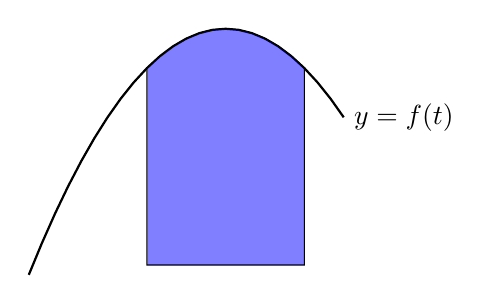
\begin{tikzpicture}
\YEtaaxis{1}{5}{1}{3}
\YExcoord{1}{a}
\YExcoord{2}{x}
\YExcoord{4}{x+h}
\draw[thick] plot[domain=.5:4.5] (\x,{3-(\x-3)*(\x-3)/2}) node[right]{$y=f(t)$};
\draw[fill=blue, fill opacity=0.5] plot[domain=2:4] (\x,{3-(\x-3)*(\x-3)/2}) |-(2,0)--cycle;
\end{tikzpicture}
\end{center}
\end{answer}
\begin{solution}

Using the definition of $F$, $\textcolor{red}{F(x)}$ is the area under the curve from $a$ to $x$, and $\textcolor{blue}{F(x+h)}$ is the area under the curve from $a$ to $x+h$. These are shown on the same diagram, below.

\begin{center}
\begin{tikzpicture}
\YEtaaxis{1}{5}{1}{3}
\YExcoord{1}{a}
\YExcoord{2}{x}
\YExcoord{4}{x+h}
\draw[thick] plot[domain=.5:4.5] (\x,{3-(\x-3)*(\x-3)/2}) node[right]{$y=f(t)$};
\draw[pattern=north east lines, pattern color=blue] plot[domain=1:4] (\x,{3-(\x-3)*(\x-3)/2}) |-(1,0)--cycle;
\draw[pattern color=red, pattern=north west lines,  opacity=0.5] plot[domain=1:2] (\x,{3-(\x-3)*(\x-3)/2}) |-(1,0)--cycle;
\end{tikzpicture}
\end{center}

Then the area represented by $\textcolor{blue}{F(x+h)}-\textcolor{red}{F(x)}$ is the area that is outside the red, but inside the blue. Equivalently, it is $\int\limits_{x}^{x+h} f(t)\ \dee{t}$.

\begin{center}
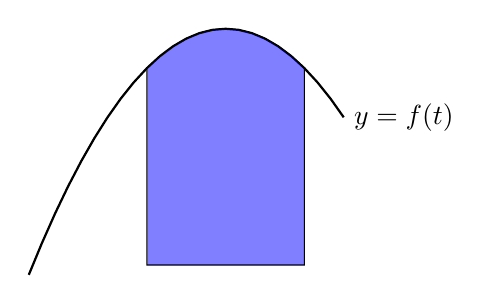
\begin{tikzpicture}
\YEtaaxis{1}{5}{1}{3}
\YExcoord{1}{a}
\YExcoord{2}{x}
\YExcoord{4}{x+h}
\draw[thick] plot[domain=.5:4.5] (\x,{3-(\x-3)*(\x-3)/2}) node[right]{$y=f(t)$};
\draw[fill=blue, fill opacity=0.5] plot[domain=2:4] (\x,{3-(\x-3)*(\x-3)/2}) |-(2,0)--cycle;
\end{tikzpicture}
\end{center}
\end{solution}
%%%%%%%%%%%%%%%%%%
\begin{Mquestion}\label{1.1_intpic1}
Let $F(x) = \displaystyle\int_0^x f(t)dt$, where $f(t)$ is shown in the graph below, and $0 \leq x \leq 4$.
\begin{enumerate}[(a)]
\item Is $F(0)$ positive, negative, or zero?
\item Where is $F(x)$ increasing and where is it decreasing?
\end{enumerate}
\begin{center}
\begin{tikzpicture}
\YEtaaxis{1}{5}{3}{3}
\draw[thick] plot[domain=-1:4.3, samples=60] (\x,{(\x+.5)*(\x-1)*(\x-3)/(abs(\x)+1)});
\foreach \x in {1,...,4}{\YExcoord{\x}{\x}}
\draw (4,2) node[right] {$y=f(t)$};
\end{tikzpicture}
\end{center}
\end{Mquestion}
\begin{hint}
$F(x)$ represents net \emph{signed} area.
\end{hint}
\begin{answer}
(a) zero \qquad (b) increasing when $0 < x < 1$ and $3<x<4$; decreasing when $1<x<3$
\end{answer}
\begin{solution}
We evaluate $F(0)$ using the definition: $F(0) = \int_0^0 f(t)\ \dee{t}=0$. Although $f(0)>0$, the \emph{area} from $t=0$ to $t=0$ is zero.\\
As $x$ moves along, $F(x)$ adds bits of signed area. If it's adding positive area, it's increasing, and if it's adding negative area, it's decreasing. So, $F(x)$ is increasing when $0 < x < 1$ and $3<x<4$, and $F(x)$ is decreasing when $1<x<3$.
\end{solution}

%%%%%%%%%%%%%%%%%%
\begin{question}
Let $G(x) = \displaystyle\int_x^0 f(t)dt$, where $f(t)$ is shown in the graph below, and $0 \leq x \leq 4$.
\begin{enumerate}[(a)]
\item Is $G(0)$ positive, negative, or zero?
\item Where is $G(x)$ increasing and where is it decreasing?
\end{enumerate}
\begin{center}
\begin{tikzpicture}
\YEtaaxis{1}{5}{3}{3}
\draw[thick] plot[domain=-1:4.3, samples=60] (\x,{(\x+.5)*(\x-1)*(\x-3)/(abs(\x)+1)});
\foreach \x in {1,...,4}{\YExcoord{\x}{\x}}
\draw (4,2) node[right] {$y=f(t)$};
\end{tikzpicture}
\end{center}
\end{question}
\begin{hint}
Note $G(x)=-F(x)$, when $F(x)$ is defined as in Question~\ref{1.1_intpic1}.
\end{hint}
\begin{answer}
(a) zero \qquad (b) $G(x)$ is increasing when $1<x<3$, and it is decreasing when $0<x<1$ and when $3<x<4$.
\end{answer}
\begin{solution}
This question is nearly identical to Question~\ref{1.1_intpic1}, with
\[G(x) = \displaystyle\int_x^0 f(t)\ \dee{t} = -\displaystyle\int_0^x f(t)\ \dee{t}=-F(x).\]
So, $G(x)$ increases when $F(x)$ decreases, and vice-versa. Therefore: $G(0)=0$, $G(x)$ is increasing when $1<x<3$, and $G(x)$ is decreasing when $0<x<1$ and when $3<x<4$.
\end{solution}

%%%%%%%%%%%%%%%%%%
\begin{question}\label{1.1_FTC2} Let $F(x) = \displaystyle\int_a^x t\ \dee{t}$.
Using the definition of the derivative, find $F'(x)$.
\end{question}
\begin{hint} Using the definition of the derivative, $F'(x) = \displaystyle\lim_{h \to 0}\dfrac{F(x+h)-F(x)}{h}$.

The area of a trapezoid with base $b$ and heights $h_1$ and $h_2$ is $\frac{1}{2}b(h_1+h_2)$.
\end{hint}
\begin{answer}
Using the definition of the derivative,
\begin{align*} F'(x) & = \displaystyle\lim_{h \to 0}\dfrac{F(x+h)-F(x)}{h}\\
&=\lim_{h \to 0}\dfrac{\int_a^{x+h} t\ \dee{t}-\int_a^x t\ \dee{t}}{h}\\
&=\lim_{h \to 0}\dfrac{\int_x^{x+h} t\ \dee{t}}{h}
\intertext{The numerator describes the area of a trapezoid with base $h$ and heights $x$ and $x+h$.}
&=\lim_{h \to 0}\dfrac{\frac{1}{2}h(x+x+h)}{h}\\
&=\lim_{h \to 0}\left(x+\frac{1}{2}h\right)\\
&=x
\end{align*}

\begin{center}
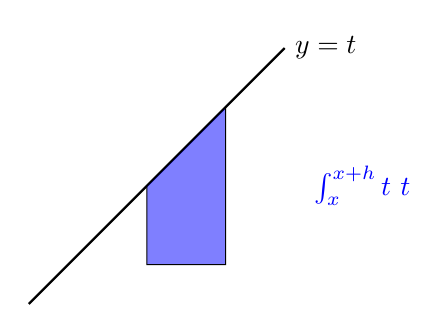
\begin{tikzpicture}
\YEtaaxis{1}{3}{1}{3}
\YExcoord{1}{x}
\YExcoord{2}{x+h}
\YEycoord{1}{x}
\YEycoord{2}{x+h}
\draw[thick] (-.5,-.5)--(2.75,2.75) node[right]{$y=t$};
\draw[fill=blue, fill opacity=0.5] (1,0)--(1,1)--(2,2)--(2,0)--cycle;
\draw[blue] (3,1) node[right]{$\int_x^{x+h}t\ \dee t$};
\end{tikzpicture}
\end{center}
So, $F'(x)=x$.
\end{answer}
\begin{solution}
Using the definition of the derivative,
\begin{align*} F'(x) & = \displaystyle\lim_{h \to 0}\dfrac{F(x+h)-F(x)}{h}\\
&=\lim_{h \to 0}\dfrac{\int_a^{x+h} t\ \dee{t}-\int_a^x t\ \dee{t}}{h}\\
&=\lim_{h \to 0}\dfrac{\int_x^{x+h} t\ \dee{t}}{h}
\intertext{The numerator describes the area of a trapezoid with base $h$ and heights $x$ and $x+h$.}
&=\lim_{h \to 0}\dfrac{\frac{1}{2}h(x+x+h)}{h}\\
&=\lim_{h \to 0}\left(x+\frac{1}{2}h\right)\\
&=x
\end{align*}
\begin{center}
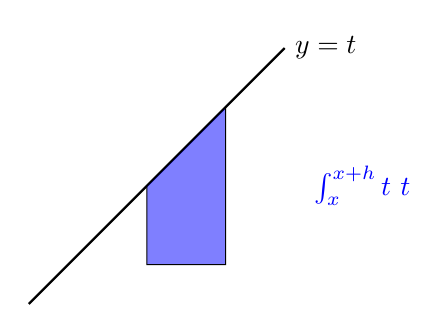
\begin{tikzpicture}
\YEtaaxis{1}{3}{1}{3}
\YExcoord{1}{x}
\YExcoord{2}{x+h}
\YEycoord{1}{x}
\YEycoord{2}{x+h}
\draw[thick] (-.5,-.5)--(2.75,2.75) node[right]{$y=t$};
\draw[fill=blue, fill opacity=0.5] (1,0)--(1,1)--(2,2)--(2,0)--cycle;
\draw[blue] (3,1) node[right]{$\int_x^{x+h}t\ \dee t$};
\end{tikzpicture}
\end{center}
So, $F'(x)=x$.
\end{solution}

%%%%%%%%%%%%%%%%%%%
\begin{question}
Give a continuous function $f(x)$ so that $F(x) = \displaystyle\int_0^x f(t)dt$ is a constant.
\end{question}
\begin{hint}
There is only one!
\end{hint}
\begin{answer}
$f(t)=0$
\end{answer}
\begin{solution}
If $F(x)$ is constant, then $F'(x)=0$. By the Fundamental Theorem of Calculus Part 1, $F'(x)=f(x)$. So, the only possible continuous function fitting the question is $f(x)=0$.

This makes intuitive sense: if moving $x$ doesn't add or subtract area under the curve, then there must not be any area under the curve--the curve should be the same as the $x$-axis.

As an aside, we mention that there are other, \emph{non-continuous} functions $f(t)$ such that $\int_0^x f(t)\ \dee{t} = 0$ for all $x$. For example, $f(t) = \left\{\begin{array}{cc}
0 & x \neq 0\\
1 & x=0
\end{array}\right.$. These kinds of removable discontinuities will not factor heavily in our discussion of integrals.
\end{solution}

%%%%%%%%%%%%%%%%%%
\Instructions{So far, we have been able to guess many antiderivatives. Often, however, antiderivatives are very difficult to guess. In Questions~\ref{1.3_inttablea} through \ref{1.3_inttableb}, we will find some antiderivatives that might appear in a table of integrals. Coming up with the antiderivative might be quite difficult (strategies to do just that will form a large part of this semester), but \emph{verifying} that your antiderivative is correct is as simple as differentiating.}
\begin{question}\label{1.3_inttablea} Evaluate and simplify $\diff{}{x}\{x\log(ax)-x\}$, where $a$ is some constant and $\log(x)$ is the logarithm base $e$. What \emph{antiderivative} does this tell you?
\end{question}
\begin{hint}
If $\diff{}{x}\{F(x)\}=f(x)$, that tells us $\int f(x)\ \dee{x} = F(x)+C$.
\end{hint}
\begin{answer}
$\int \log(ax)\ \dee{x}= x\log(ax)-x+C$, where $a$ is a given constant, and $C$ is any constant.
\end{answer}
\begin{solution}
\begin{align*}
\diff{}{x}\{x\log(ax)-x\}&=x\left(\frac{a}{ax}\right)+\log(ax)-1 &\mbox{(product rule, chain rule)}\\
&=\log(ax)
\intertext{So, we know}
\int \log(ax)\ \dee{x}&= x\log(ax)-x+C&\mbox{where $a$ is a given constant, and $C$ is any constant.}
\end{align*}
Remark: $\int \log(ax)\ \dee{x}$ can be calculated using the method of Integration by Parts, which you will learn in Section~\eref{CLP101}{sec intbyparts} of the CLP-2 text.
\end{solution}
%%%%%%%%%%%%%%%%%%
\begin{question} Evaluate and simplify $\diff{}{x}\{e^x\left(x^3-3x^2+6x-6\right)\}$. What \emph{antiderivative} does this tell you?
\end{question}
\begin{hint}
When you're differentiating, you can leave the $e^x$ factored out.
\end{hint}
\begin{answer}
$\int x^3e^x\ \dee{x}=e^x\left(x^3-3x^2+6x-6\right)+C
$
\end{answer}
\begin{solution}
\begin{align*}
\diff{}{x}\left\{e^x\left(x^3-3x^2+6x-6\right)\right\}&=e^x\left(3x^2-6x+6\right)+e^x\left(x^3-3x^2+6x-6\right)
&\mbox{(product rule)}\\
&=e^x\left(3x^2-6x+6+x^3-3x^2+6x-6\right)\\
&=x^3e^x
\intertext{So,}
\int x^3e^x\ \dee{x}&=e^x\left(x^3-3x^2+6x-6\right)+C
\end{align*}

Remark: $\int x^3e^x\ \dee{x}$ can be calculated using the method of Integration by Parts, which you will learn in Section~\eref{CLP101}{sec intbyparts} of the CLP-2 text.

\end{solution}
%%%%%%%%%%%%%%%%%%
\begin{question} Evaluate and simplify $\diff{}{x}\left\{\log\left|x+\sqrt{x^2+a^2}\right|\right\}$, where $a$ is some constant. What \emph{antiderivative} does this tell you?
\end{question}
\begin{hint}
After differentiation, you can simplify pretty far. Keep at it!
\end{hint}
\begin{answer}
$\displaystyle\int \dfrac{1}{\sqrt{x^2+a^2}}\ \dee{x} = \log\left|x+\sqrt{x^2+a^2}\right|+C
$ when $a$ is a given constant. As usual, $C$ is an arbitrary constant.
\end{answer}
\begin{solution}
\begin{align*}
\diff{}{x}\left\{\log\left|x+\sqrt{x^2+a^2}\right|\right\}&=
\frac{1}{x+\sqrt{x^2+a^2}}\cdot \left(1+\frac{1}{2\sqrt{x^2+a^2}}\cdot 2x\right)
&\mbox{(chain rule)}\\
&=\frac{1+\frac{x}{\sqrt{x^2+a^2}}}{x+\sqrt{x^2+a^2}}
=\frac{\frac{\sqrt{x^2+a^2}+x}{\sqrt{x^2+a^2}}}{x+\sqrt{x^2+a^2}}\\
&=\frac{1}{\sqrt{x^2+a^2}}
\intertext{So,}
\int \frac{1}{\sqrt{x^2+a^2}}\ \dee{x} &= \log\left|x+\sqrt{x^2+a^2}\right|+C
\end{align*}

Remark: $\int \frac{1}{\sqrt{x^2+a^2}}\ \dee{x} $ can be calculated using the method of Trigonometric Substitution, which you will learn in Section~\eref{CLP101}{sec trigsub}
of the CLP-2 text.

\end{solution}
%%%%%%%%%%%%%%%%%%
\begin{question}\label{1.3_inttableb} Evaluate and simplify $\displaystyle\diff{}{x}\left\{\sqrt{x(a+x)}-a\log\left(\sqrt{x}+\sqrt{a+x}\right)\right\}$, where $a$ is some constant. What \emph{antiderivative} does this tell you?
\end{question}
\begin{hint} This derivative also simplifies considerably. You might need to add fractions by finding a common denominator.
\end{hint}
\begin{answer}
$\displaystyle\int \dfrac{x}{\sqrt{x(a+x)}}\ \dee{x}=\sqrt{x(a+x)}-a\log\left(\sqrt{x}+\sqrt{a+x}\right)+C$
\end{answer}
\begin{solution}
Using the chain rule:
\begin{align*}
\diff{}{x}&\left\{\sqrt{x(a+x)}-a\log\left(\sqrt{x}+\sqrt{a+x}\right)\right\}\\
&=
\frac{x+(a+x)}{2\sqrt{x(a+x)}}-a\left(\frac{1}{\sqrt{x}+\sqrt{a+x}}\cdot\left(\frac{1}{2\sqrt{x}}+\frac{1}{2\sqrt{a+x}}\right)\right)
\\&=
\frac{2x+a}{2\sqrt{x(a+x)}}-
a\left(
\frac{1}{\sqrt{x}+\sqrt{a+x}}\cdot\left(
\frac{\sqrt{a+x}+\sqrt{x}}{2\sqrt{x(a+x)}}\right)\right)
\\&=
\frac{2x+a}{2\sqrt{x(a+x)}}-
a\left(\frac{1}{2\sqrt{x(a+x)}}\right)\\
&=\frac{2x}{2\sqrt{x(a+x)}} = \frac{x}{\sqrt{x(a+x)}}
\intertext{So,}
\int \frac{x}{\sqrt{x(a+x)}}\ \dee{x}&=\sqrt{x(a+x)}-a\log\left(\sqrt{x}+\sqrt{a+x}\right)+C
\end{align*}

Remark: $\int \frac{x}{\sqrt{x(a+x)}}\ \dee{x}$ can be calculated using the method of Trigonometric Substitution, which you will learn in Section~\eref{CLP101}{sec trigsub}
of the CLP-2 text.

\end{solution}

%%%%%%%%%%%%%%%%%%
\subsection*{\Procedural}
%%%%%%%%%%%%%%%%%%

\begin{Mquestion}[2016Q2]
Evaluate $\displaystyle\int_0^2 \big(x^3+\sin x)\,\dee{x}$.
\end{Mquestion}

\begin{hint}
Guess a function whose derivative is the integrand, then use the Fundamental Theorem of Calculus Part 2.
\end{hint}

\begin{answer}
$5-\cos 2$
\end{answer}

\begin{solution}
By the Fundamental Theorem of Calculus,
\begin{align*}
\int_0^2 \big(x^3+\sin x)\,\dee{x}
&=\left[\frac{x^4}{4}-\cos x\right]_0^2\\
&=\left(\frac{2^4}{4}-\cos 2\right)-\left(0 -\cos 0\right) \\
&= 4-\cos2+1=5-\cos2.
\end{align*}

\end{solution}
%%%%%%%%%%%%%%%%%%%


\begin{question}[2012A]
Evaluate $\displaystyle\int_1^2 \frac{x^2+2}{x^2}\,\dee{x}$.
\end{question}

\begin{hint}
Split the given integral up into two integrals.
\end{hint}

\begin{answer}
$2$
\end{answer}

\begin{solution}
By part (d) of our ``Arithmetic of Integration'' theorem, Theorem \eref{CLP101}{thm:Intarith}
in the CLP-2 text,
\begin{equation*}
\int_1^2 \frac{x^2+2}{x^2}\,\dee{x}
=\int_1^2 \Big[1+\frac{2}{x^2}\Big]\,\dee{x}
=\int_1^2 \dee{x} + 2\int_1^2 \frac{1}{x^2}\,\dee{x}
\end{equation*}
Then by the Fundamental Theorem of Calculus Part 2,
\begin{align*}
\int_1^2 \dee{x} + 2\int_1^2 \frac{1}{x^2}\,\dee{x}
=\Big[x\Big]_1^2 + 2\Big[-\frac{1}{x}\Big]_1^2
=\big[2-1\big] + 2\Big[-\frac{1}{2}+1\Big]
=2
\end{align*}

\end{solution}
%%%%%%%%%%%%%%%%%%%

%%%%%%%%%%%%%%%%%%
\begin{question}
Evaluate $\displaystyle\int \dfrac{1}{1+25x^2}\dee{x}$.
\end{question}
\begin{hint}
The integrand is similar to $\dfrac{1}{1+x^2}$, so something with arctangent seems in order.
\end{hint}
\begin{answer}
$\dfrac{1}{5}\arctan(5x)+C$
\end{answer}
\begin{solution}
The integrand is similar to $\dfrac{1}{1+x^2}$, which is the derivative of arctangent. Indeed, we have
\begin{align*}\displaystyle\int \dfrac{1}{1+25x^2}\dee{x} &= \int \dfrac{1}{1+(5x)^2}\dee{x}.
\intertext{ So, a reasonable first guess for the antiderivative might be }
\color{red}F(x) &\color{red}\stackrel{?}{=} \arctan(5x).
\intertext{ However, because of the chain rule, }
\color{red}F'(x) &\color{red}= \dfrac{5}{1+(5x)^2}.
\intertext{ In order to ``fix" the numerator, we make a second guess: }
\color{blue}F(x) &\color{blue}= \frac{1}{5}\arctan(5x)\\
\color{blue}F'(x) &\color{blue}= \dfrac{1}{5}\left(\dfrac{5}{1+(5x)^2}\right) = \dfrac{1}{1+25x^2}\\
 \mbox{So,}\qquad
\displaystyle\int \dfrac{1}{1+25x^2}\dee{x}&=\frac{1}{5}\arctan(5x)+C.
\end{align*}
\end{solution}

%%%%%%%%%%%%%%%%%%
\begin{question}
Evaluate $\displaystyle\int \dfrac{1}{\sqrt{2-x^2}}\dee{x}$.
\end{question}
\begin{hint}
The integrand is similar to $\dfrac{1}{\sqrt{1-x^2}}$, so factoring out $\sqrt{2}$ from the denominator will make it look like some flavour of arcsine.
\end{hint}
\begin{answer}
$\arcsin\left(\dfrac{x}{\sqrt{2}}\right)+C$
\end{answer}
\begin{solution}
The integrand is similar to $\dfrac{1}{\sqrt{1-x^2}}$. In order to formulate a guess for the antiderivative, let's factor out $\sqrt{2}$ from the denominator:
\begin{align*}
\displaystyle\int \dfrac{1}{\sqrt{2-x^2}}\dee{x}&=
\displaystyle\int \dfrac{1}{\sqrt{2\left(1-\frac{x^2}{2}\right)}}\dee{x}\\
&=\displaystyle\int \dfrac{1}{
\sqrt{2}\sqrt{1-\frac{x^2}{2}}}\dee{x}\\
&=
\int\frac{1}{\sqrt{2}}\cdot \dfrac{1}{
\sqrt{1-\left(\dfrac{x}{\sqrt2}\right)^2}}\dee{x}\\
\intertext{At this point, we might guess that our antiderivative is something like $F(x) = \arcsin\left(\dfrac{x}{\sqrt{2}}\right)$. To explore this possibility, we can differentiate, and see what we get.}
\diff{}{x}\left\{\arcsin\left(\dfrac{x}{\sqrt{2}}\right)\right\}&=\frac{1}{\sqrt{2}}\cdot\dfrac{1}{\sqrt{1-\left(\dfrac{x}{\sqrt{2}}\right)^2}}
\intertext{This is exactly what we want! So,}
\int \dfrac{1}{\sqrt{2-x^2}}\dee{x}&=\arcsin\left(\dfrac{x}{\sqrt2}\right)+C
\end{align*}

\end{solution}
%%%%%%%%%%%%%%%%%%
\begin{question} Evaluate $\displaystyle\int \tan^2 x \ \dee{x}$.
\end{question}
\begin{hint}
We know how to antidifferentiate $\sec^2 x$, and there is an identity linking $\sec^2 x$ with $\tan^2 x$.
\end{hint}
\begin{answer}
$\tan x - x +C$
\end{answer}
\begin{solution}
We know that $\int \sec^2 x\ \dee{x} = \tan x +C$, and $\sec^2x = \tan^2 x + 1$, so
\begin{align*}
\int \tan^2 x\ \dee{x} &= \int \sec^2x - 1 \ \dee{x}\\
&=\int \sec^2 x \ \dee{x} - \int 1 \ \dee{x}\\
&=\tan x - x + C
\end{align*}
\end{solution}
%%%%%%%%%%%%%%%%%%
\begin{question} Evaluate $\displaystyle\int 3 \sin x \cos x \ \dee{x}$.
\end{question}
\begin{hint} Recall $2\sin x \cos x = \sin(2x)$.
\end{hint}
\begin{answer}
$-\dfrac{3}{4}\cos(2x)+C$, or
 equivalently,
$\dfrac{3}{2}\sin^2 x+C$
\end{answer}
\begin{solution}
\begin{description}
\item[Solution 1:] This might not obviously look like the derivative of anything familiar, but it does look like half of a familiar trig identity:
$2\sin x \cos x = \sin(2x)$.
\begin{align*}
\int 3 \sin x \cos x \ \dee{x}&=\int \frac{3}{2}\cdot 2\sin x \cos x \ \dee{x}\\
&=\int \frac{3}{2} \sin(2x)\ \dee{x}
\intertext{So, we might guess that the antiderivative is something like $-\cos(2x)$. We only need to figure out the constants.}
\diff{}{x}\{-\cos(2x)\}&=2\sin(2x)\\
\mbox{So,}\qquad
\diff{}{x}\left\{-\frac{3}{4}\cos(2x)\right\}&=\frac{3}{2}\sin(2x)\\
\mbox{Therefore,}\qquad \int 3\sin x \cos x\ \dee{x}&=-\frac{3}{4}\cos(2x)+C
\end{align*}
\item[Solution 2:]
You might notice that the integrand looks  like it came from the chain rule, since $\cos x$ is the derivative of $\sin x$. Using this observation, we can work out the antideriative:
\begin{align*}
\diff{}{x}\left\{\sin^2 x\right\}&=2\sin x \cos x\\
\diff{}{x}\left\{\frac{3}{2}\sin^2 x\right\}&=3\sin x \cos x\\
\mbox{So,}\qquad \int 3\sin x \cos x \ \dee{x}&=\frac{3}{2}\sin^2 x+C
\end{align*}
\end{description}
These two answers look different. Using the identity $\cos(2x)=1 - 2 \sin^2(x)$, we reconcile them:
\begin{align*}
-\frac{3}{4}\cos(2x)+C&= -\frac{3}{4}\left(1-2\sin^2x\right)+C\\
&=\frac{3}{2}\sin^2 x + \left(C-\frac{3}{4}\right)
\end{align*}
 The $\frac{3}{4}$ here is not significant. Remember that $C$ is  used
         to designate a constant that can take any value between $-\infty$ and $+\infty$.
         So $C-\frac{3}{4}$ is also just a constant that can take any value between
         $-\infty$ and $+\infty$. As the two answers we found differ by a constant,
         they are equivalent.\end{solution}
%%%%%%%%%%%%%%%%%%
\begin{question} Evaluate $\displaystyle\int \cos^2 x \ \dee{x}$.
\end{question}
\begin{hint}
$\cos^2 x = \dfrac{1+\cos(2x)}{2}$
\end{hint}
\begin{answer}
$\dfrac{1}{2}x+\dfrac{1}{4}\sin(2x)+C$
\end{answer}
\begin{solution}
It's not immediately obvious which function has $\cos^2 x$ as its derivative, but we can make the situation a little clearer by using the identity $\cos^2 x = \dfrac{1+\cos(2x)}{2}$:
\begin{align*}
\int \cos^2 x \ \dee{x}&=\int \frac{1}{2}\cdot \left(1+\cos(2x)\right)\ \dee{x}\\
&=\int \frac{1}{2}\ \dee{x} + \int \frac{1}{2}\cos(2x)\ \dee{x}\\
&=\frac{1}{2}x + C+  \int \frac{1}{2}\cos(2x)\ \dee{x}
\intertext{For the remaining integral, we might guess something like $F(x) = \sin(2x)$. Let's figure out the appropriate constant:}
\diff{}{x}\left\{ \sin(2x) \right\}&=2\cos(2x)\\
\diff{}{x}\left\{ \frac{1}{4}\sin(2x) \right\}&=\frac{1}{2}\cos(2x)\\
\mbox{So,}\qquad
 \int \frac{1}{2}\cos(2x)\ \dee{x} &=\frac{1}{4}\sin(2x)+C\\
\mbox{Therefore,}\qquad
 \int \cos^2 x \ \dee{x}&=\frac{1}{2}x+\frac{1}{4}\sin(2x)+C
\end{align*}
\end{solution}
%%%%%%%%%%%%%%%%%%

\begin{question}[M105 2012A]
If
\begin{equation*}
F(x)=\int_0^x \log(2+\sin t)\,\dee{t}\quad\text{and}\quad
G(y)=\int^0_y \log(2+\sin t)\,\dee{t}
\end{equation*}
find $F'\big(\frac{\pi}{2}\big)$ and $G'\big(\frac{\pi}{2}\big)$.
\end{question}

%\begin{hint}
%\end{hint}

\begin{answer}
$F'\left(\frac{\pi}{2}\right)=\log(3)$\qquad
$G'\left(\frac{\pi}{2}\right)=-\log(3)$
\end{answer}

\begin{solution}
By the Fundamental Theorem of Calculus Part 1,
\begin{alignat*}{3}
F'(x)&=\diff{}{x} \int_0^x \log(2+\sin t)\,\dee{t}
     &&=\log(2+\sin x) \\
G'(y)&=\diff{}{y}\bigg[- \int_0^y \log(2+\sin t)\,\dee{t}\bigg]
     &&=-\log(2+\sin y) \\
\end{alignat*}
So,
\begin{equation*}
F'\Big(\frac{\pi}{2}\Big)=\log 3\qquad
G'\Big(\frac{\pi}{2}\Big)=-\log(3)
\end{equation*}
\end{solution}
%%%%%%%%%%%%%%%%%%%



\begin{Mquestion}[2014A]
Let $f(x)=\displaystyle\int_1^x 100(t^2-3t+2)e^{-t^2}\ \dee{t}$.
Find the interval(s) on which $f$ is increasing.
\end{Mquestion}

\begin{hint}
There is a good way to test where a function is increasing,
decreasing, or constant, that also has something to do with topic
of this section.
\end{hint}

\begin{answer}
$f(x)$ is increasing when
$-\infty<x<1$ and when $2<x<\infty$.
\end{answer}

\begin{solution}
By the Fundamental Theorem of Calculus Part 1,
\begin{equation*}
f'(x) = 100(x^2-3x+2)e^{-x^2}
      = 100(x-1)(x-2)e^{-x^2}
\end{equation*}
As $f(x)$ is increasing whenever $f'(x)>0$ and $100 e^{-x^2}$
is always strictly bigger than $0$,
we have $f(x)$ increasing if and only if $(x-1)(x-2)>0$, which
is the case if and only if $(x-1)$ and $(x-2)$ are of the same
sign. Both are positive when $x>2$ and both are negative when
$x<1$. So $f(x)$ is increasing when
$-\infty<x<1$ and when $2<x<\infty$.

Remark: even without the Fundamental Theorem of Calculus, since $f(x)$ is the area under a curve from 1 to $x$, $f(x)$ is increasing when the curve is above the $x$-axis (because we're adding positive area), and it's decreasing when the curve is below the $x$-axis (because we're adding negative area).
\end{solution}
%%%%%%%%%%%%%%%%%%%

\begin{Mquestion}[M105 2013A]
If $F(x)={\displaystyle\int_0^{\cos x} \frac{1}{t^3+6}\,\dee{t}}$,
find $F'(x)$.
\end{Mquestion}

\begin{hint}
See Example \eref{CLP101}{eg:INTftocB} in the
%\href{http://www.math.ubc.ca/%7Efeldman/m101/clp/clp_notes_101.pdf#section1.6}{CLP 101 notes}.
%\href{http://www.math.ubc.ca/%7Efeldman/m101/clp/clp_notes_101.pdf}{CLP 101 notes}.
CLP-2 text.
\end{hint}

\begin{answer}
$F'(x)=-\dfrac{\sin x}{\cos^3x+6}$
\end{answer}

\begin{solution}
Write $G(x)={\displaystyle\int_0^x \frac{1}{t^3+6}\,\dee{t}}$.
By the Fundamental Theorem of Calculus Part 1, $G'(x)=\dfrac{1}{x^3+6}$.
Since $F(x)=G(\cos x)$, the chain rule gives us
\begin{align*}
F'(x)=G'(\cos x)\cdot(-\sin x)=-\frac{\sin x}{\cos^3x+6}
\end{align*}
\end{solution}
%%%%%%%%%%%%%%%%%%%



\begin{question}[1997D]
 Compute $f'(x)$ where $f(x)= \displaystyle\int_0^{1+x^4}e^{t^2}\dee{t}$.
\end{question}

\begin{hint}
See Example \eref{CLP101}{eg:INTftocB} in the
%\href{http://www.math.ubc.ca/%7Efeldman/m101/clp/clp_notes_101.pdf#section1.6}{CLP 101 notes}.
%\href{http://www.math.ubc.ca/%7Efeldman/m101/clp/clp_notes_101.pdf}{CLP 101 notes}.
CLP-2 text.
\end{hint}

\begin{answer}
$4x^3e^{(1+x^4)^2}$
\end{answer}

\begin{solution}
Define $g(x)= \displaystyle\int_0^x e^{t^2}\dee{t}$. By the Fundamental
Theorem of Calculus Part 1, $g'(x)=e^{x^2}$. As $f(x)=g(1+x^4)$
the chain rule gives us
\begin{align*}
f'(x)=4x^3g'(1+x^4)=4x^3e^{(1+x^4)^2}
\end{align*}
\end{solution}
%%%%%%%%%%%%%%%%%%%

\begin{question}[M105 2015A]
 Evaluate $\displaystyle\diff{}{x}\left\{\int_0^{\sin x}(t^6+8)\dee{t}\right\}$.
\end{question}

\begin{hint}
See Example \eref{CLP101}{eg:INTftocB} in the
%\href{http://www.math.ubc.ca/%7Efeldman/m101/clp/clp_notes_101.pdf#section1.6}{CLP 101 notes}.
%\href{http://www.math.ubc.ca/%7Efeldman/m101/clp/clp_notes_101.pdf}{CLP 101 notes}.
CLP-2 text.
\end{hint}

\begin{answer}
$\big(\sin^6 x+8)\cos x$
\end{answer}

\begin{solution}
Define $g(x)=\int_0^x (t^6+8)\dee{t}$. By the fundamental
theorem of calculus, $g'(x)=x^6+8$. We are to compute the derivative of $f(x)=g(\sin x)$. The chain rule gives
\begin{align*}
\diff{}{x}\left\{\int_0^{\sin x}(t^6+8)\dee{t}\right\}
  =g'(\sin x)\cdot \cos x=\big(\sin^6 x+8\big)\cos x
\end{align*}
\end{solution}
%%%%%%%%%%%%%%%%%%%


\begin{question}[2000D]
Let $F(x)= \displaystyle\int_0^{x^3}e^{-t}\sin\left(\frac{\pi t}{2}\right)\,\dee{t}$.
Calculate $F'(1)$.
\end{question}

\begin{hint}
See Example \eref{CLP101}{eg:INTftocB} in the
%\href{http://www.math.ubc.ca/%7Efeldman/m101/clp/clp_notes_101.pdf#section1.6}{CLP 101 notes}.
%\href{http://www.math.ubc.ca/%7Efeldman/m101/clp/clp_notes_101.pdf}{CLP 101 notes}.
CLP-2 text.
\end{hint}

\begin{answer}
$F'(1)=3e^{-1}$
\end{answer}

\begin{solution}
Let $G(x)= \displaystyle\int_0^{x}e^{-t}\sin\left(\frac{\pi t}{2}\right)\,\dee{t}$.
By the Fundamental Theorem of Calculus Part 1,  $G'(x)=e^{-x}\sin\big(\frac{\pi x}{2}\big)$ and,
since $F(x)=G(x^3)$,
$F'(x)=3x^2G'(x^3)=3x^2e^{-x^3}\sin\big(\frac{\pi x^3}{2}\big)$. Then
$F'(1)=3e^{-1}\sin\big(\frac{\pi }{2}\big)
=3e^{-1}$.
\end{solution}
%%%%%%%%%%%%%%%%%%%%%%%%%%%%%%%%%%%%%%%%

\begin{question}[2016Q2]
Find $\displaystyle \diff{}{u} \left\{ \int_{\cos u}^0 \frac{\dee{t}}{1+t^3}
\right\}$.
\end{question}

\begin{hint}
See Example \eref{CLP101}{eg:INTftocC} in the
%\href{http://www.math.ubc.ca/%7Efeldman/m101/clp/clp_notes_101.pdf#section1.6}{CLP 101 notes}.
%\href{http://www.math.ubc.ca/%7Efeldman/m101/clp/clp_notes_101.pdf}{CLP 101 notes}.
CLP-2 text.
\end{hint}

\begin{answer}
$\displaystyle{}\frac{\sin{u}}{1+\cos^3 u}$
\end{answer}

\begin{solution}
Define $\displaystyle G(x) = \int_x^0 \frac{\dee{t}}{1+t^3}
   = - \int_0^x \frac1{1+t^3}\,\dee{t}$, so that
$\displaystyle G'(x) = - \frac1{1+x^3}$ by the Fundamental Theorem of Calculus Part 1.
Then by the chain rule,
\begin{align*}
\diff{}{u} \left\{ \int_{\cos u}^0 \frac{\dee{t}}{1+t^3} \right\}
= \diff{}{u} G(\cos u)
=  G'(\cos u) \cdot \diff{}{u}\cos u
= {-}\frac{1}{1+\cos^3 u} \cdot (-\sin{u}).
\end{align*}
\end{solution}
%%%%%%%%%%%%%%%%%%%



\begin{question}[M121 2000A]
Find  $f(x)$ if $x^2=1+\displaystyle\int_1^x f(t)\ \dee{t}$.
\end{question}

\begin{hint}
Apply $\diff{}{x}$ to both sides.
\end{hint}

\begin{answer}
$f(x)=2x$
\end{answer}

\begin{solution}
Applying $\diff{}{x}$ to both sides of
$x^2=1+\int_1^x f(t)\ \dee{t}$ gives, by the Fundamental Theorem of Calculus Part 1,
$2x=f(x)$.
\end{solution}
%%%%%%%%%%%%%%%%%%%



\begin{question}[2013A]
If $x \sin(\pi x) = \displaystyle\int_0^x f(t)\, \dee{t}$ where $f$
is a continuous function, find $f(4)$.
\end{question}

\begin{hint}
What is the title of this section?
\end{hint}

\begin{answer}
$f(4)=4\pi$

\end{answer}

\begin{solution}
Apply $\diff{}{x}$ to both sides of
$x \sin(\pi x) = \int_0^x f(t)\, \dee{t}$. Then, by the Fundamental Theorem
of Calculus Part 1,
\begin{alignat*}{3}
&&f(x)
    =\diff{}{x} \int_0^x f(t)\, \dee{t}&=\diff{}{x}\big\{x \sin(\pi x)\big\} \\
\implies&& f(x) &= \diff{}{x}\big\{x \sin(\pi x)\big\}
               =\sin(\pi x)+\pi x\cos(\pi x) \\
\implies&& f(4)&= \sin(4\pi)+4\pi\cos(4\pi)=4\pi
\end{alignat*}

\end{solution}
%%%%%%%%%%%%%%%%%%%

\begin{question}[2016Q2]
Consider the function $\displaystyle F(x)=\int_0^{x^2} e^{-t}\,\dee{t} +\int_{-x}^0 e^{-t^2}\,\dee{t}$.
\begin{enumerate}[(a)]
\item
Find $F'(x)$.
\item
Find the value of $x$ for which $F(x)$ takes its minimum value.
\end{enumerate}
\end{question}

\begin{hint}
See Example \eref{CLP101}{eg:INTftocC} in the
%\href{http://www.math.ubc.ca/%7Efeldman/m101/clp/clp_notes_101.pdf#section1.6}{CLP 101 notes}.
%\href{http://www.math.ubc.ca/%7Efeldman/m101/clp/clp_notes_101.pdf}{CLP 101 notes}.
CLP-2 text.
\end{hint}

\begin{answer}
(a) $(2x+1)e^{-x^2}$
\qquad (b) $x=-1/2$
\end{answer}

\begin{solution}
(a) Write
\begin{align*}
F(x)=G(x^2)-H(-x)\qquad\hbox{with}\quad G(y)=\int_0^{y} e^{-t}\,\dee{t},\
H(y)=\int^{y}_0 e^{-t^2}\,\dee{t}
\end{align*}
By the Fundamental Theorem of Calculus Part 1,
\begin{align*}
G'(y)=e^{-y}\, ,\qquad
H'(y)= e^{-y^2}
\end{align*}
Hence, by the chain rule,
\begin{align*}
F'(x)=2x G'(x^2)-(-1)H'(-x)=2x e^{-(x^2)}+e^{-(-x)^2}
      =(2x+1)e^{-x^2}
\end{align*}

\noindent (b) Observe that $F'(x)<0$ for $x<-1/2$ and $F'(x)>0$ for $x>-1/2$.
Hence $F(x)$ is decreasing for $x<-1/2$ and increasing for $x>-1/2$,
and $F(x)$ must take its minimum value when $x=-1/2$.

\end{solution}
%%%%%%%%%%%%%%%%%%%

\begin{question}[2016A]
If $F(x)$ is defined by
$\displaystyle F(x) = \int_{x^4-x^3}^x e^{\sin t}\,\dee{t}$, find $F'(x)$.
\end{question}

\begin{hint}
See Example \eref{CLP101}{eg:INTftocC} in the
CLP-2 text.

\end{hint}

\begin{answer}
$e^{\sin x}-e^{\sin(x^4-x^3)}\big(4x^3-3x^2\big)$
\end{answer}

\begin{solution}
Define $G(y)=\displaystyle\int_0^ye^{\sin t}\ \dee{t}$. Then:
\begin{align*}
F(x) &= \int_0^x e^{\sin t}\,\dee{t} + \int_{x^4-x^3}^0 e^{\sin t}\,\dee{t}
= \int_0^x e^{\sin t}\,\dee{t} - \int_0^{x^4-x^3} e^{\sin t}\,\dee{t} \\
&=G(x) - G(x^4-x^3)
\end{align*}

By the Fundamental Theorem of Calculus Part 1,
\begin{align*}
G'(y)=e^{\sin y}\qquad
\end{align*}
Hence, by the chain rule,
\begin{align*}
F'(x) &= G'(x)- G'(x^4-x^3)\ \diff{}{x}\big\{x^4-x^3\big\} \\
 &= G'(x)- G'(x^4-x^3)\ (4x^3-3x^2) \\
&=e^{\sin x}-e^{\sin(x^4-x^3)}\big(4x^3-3x^2\big)
\end{align*}
\end{solution}
%%%%%%%%%%%%%%%%%%%

\begin{Mquestion}[M121 2012A]
Evaluate
$\displaystyle \diff{}{x}\bigg\{\int_{x^5}^{-x^2} \cos\big(e^t\big)\,\dee{t}$\bigg\}.
\end{Mquestion}

\begin{hint}
See Example \eref{CLP101}{eg:INTftocC} in the  CLP-2 text.
\end{hint}

\begin{answer}
$-2x \cos\big(e^{-x^2}\big) -5x^4\cos\big(e^{x^5}\big)$
\end{answer}

\begin{solution}
Define
with
$G(y) = \displaystyle\int_0^y \cos\big(e^t\big)\,\dee{t}$.
Then:
\begin{align*}
F(x) &=  \int_{x^5}^{-x^2} \cos\big(e^t\big)\,\dee{t}
=\int_0^{-x^2} \cos\big(e^t\big)\,\dee{t} + \int_{x^5}^0 \cos\big(e^t\big)\,\dee{t} \\
&=\int_0^{-x^2} \cos\big(e^t\big)\,\dee{t} - \int_0^{x^5} \cos\big(e^t\big)\,\dee{t} \\
&=G(-x^2) - G(x^5)
\end{align*}
By the Fundamental Theorem of Calculus,
\begin{align*}
G'(y)=\cos\big(e^y\big)
\end{align*}
Hence, by the chain rule,
\begin{align*}
F'(x) &= G'(-x^2)\ \diff{}{x}\big\{-x^2\big\} - G'(x^5)\ \diff{}{x}\big\{x^5\big\} \\
 &= G'(-x^2)\ (-2x)- G'(x^5)\ (5x^4) \\
&=-2x \cos\big(e^{-x^2}\big) -5x^4\cos\big(e^{x^5}\big)
\end{align*}
\end{solution}
%%%%%%%%%%%%%%%%%%%

\begin{question}[2014D]
Differentiate
$\displaystyle \int_x^{e^x} \sqrt{\sin t}\,\dee{t}$ for $0<x<\log \pi$.
\end{question}

\begin{hint}
See Example \eref{CLP101}{eg:INTftocC} in the
CLP-2 text.
\end{hint}

\begin{answer}
$e^x\sqrt{\sin(e^x)} -\sqrt{\sin(x)}$
\end{answer}

\begin{solution}
Define
with
$G(y) = \displaystyle\int_0^y \sqrt{\sin t}\,\dee{t}$.
Then:
\begin{align*}
F(x)&=\int_x^{e^x} \sqrt{\sin t}\,\dee{t} \\
&= \int_0^{e^x} \sqrt{\sin t}\,\dee{t} + \int_x^0 \sqrt{\sin t}\,\dee{t}
= \int_0^{e^x} \sqrt{\sin t}\,\dee{t} - \int_0^x \sqrt{\sin t}\,\dee{t} \\
&=G(e^x) - G(x)
\end{align*}
By the Fundamental Theorem of Calculus Part 1,
\begin{align*}
G'(y)=\sqrt{\sin y}\qquad
\end{align*}
Hence, by the chain rule,
\begin{align*}
F'(x) &= G'(e^x)\ \diff{}{x}\big\{e^x\big\} - G'(x)\\
 &=  e^xG'(e^x) - G'(x)\\
&=e^x\sqrt{\sin(e^x)} -\sqrt{\sin(x)}
\end{align*}
\end{solution}
%%%%%%%%%%%%%%%%%%%



\begin{question}[M105 2014A]
Evaluate $\displaystyle \int_1^5 f(x)\,\dee{x}$, where
$\displaystyle f(x)= \begin{cases} 3 &\text{ if $x\le 3$} \\
                                   x &\text{ if $x\ge 3$}
                     \end{cases}$.
\end{question}

\begin{hint}
Split up the domain of integration.
\end{hint}

\begin{answer}
$14$
\end{answer}

\begin{solution}
Splitting up the domain of integration,
\begin{align*}
 \int_1^5 f(x)\ \dee{x}
&= \int_1^3 f(x)\,\dee{x}   +  \int_3^5 f(x)\,\dee{x} \\
&= \int_1^3  3\,\dee{x}   +  \int_3^5 x\,\dee{x} \\
&= 3x\bigg|_{x=1}^{x=3} +\frac{x^2}{2} \bigg|_{x=3}^{x=5} \\
&=14
\end{align*}

\begin{center}
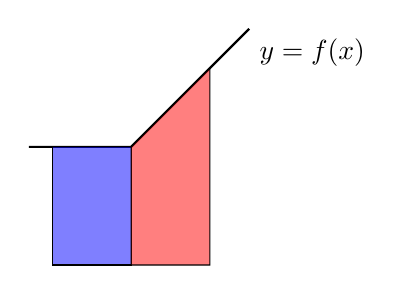
\begin{tikzpicture}
\YEaaxis{1}{4}{.25}{3}
\YExcoord{.5}{1}
\YExcoord{1.5}{3}
\YExcoord{2.5}{5}
\YEycoord{1.5}{3}
\draw[thick] (.2,1.5)--(1.5,1.5)--(3,3) node[below right]{$y=f(x)$};
\draw[fill=blue, fill opacity=0.5] (.5,0)rectangle (1.5,1.5);
\draw[fill=red, fill opacity=0.5] (1.5,0) -| (2.5,2.5)--(1.5,1.5)--cycle;
\end{tikzpicture}
\end{center}

\end{solution}
%%%%%%%%%%%%%%%%%%%




%%%%%%%%%%%%%%%%%%
\subsection*{\Application}
%%%%%%%%%%%%%%%%%%


\begin{question}[M105 2014A]
If $f'(1)=2$ and $f'(2)=3$, find $\displaystyle\int_1^2 f'(x) f''(x)\,\dee{x}$.
\end{question}

\begin{hint}
It is possible to guess an antiderivative for $f'(x) f''(x)$
that is expressed in terms of $f'(x)$.
\end{hint}

\begin{answer}
$\dfrac{5}{2}$
\end{answer}

\begin{solution}
By the chain rule,
\begin{align*}
\diff{}{x}\big\{\left(f'(x)\right)^2\big\} = 2 f'(x)\,f''(x)
\end{align*}
so $\frac{1}{2} f'(x)^2$ is an antiderivative for $f'(x)\,f''(x)$ and,
by the Fundamental Theorem of Calculus Part 2,
\begin{align*}
\int_1^2 f'(x) f''(x)\,\dee{x}
=\left[\frac{1}{2}\left(f'(x)\right)^2\right]_{x=1}^{x=2}
=\frac{1}{2} f'(2)^2 - \frac{1}{2} f'(1)^2
=\frac{5}{2}
\end{align*}

Remark: evaluating antiderivatives of this type will occupy the next section, Section~\eref{CLP101}{sec subs} of the CLP-2 text.
\end{solution}
%%%%%%%%%%%%%%%%%%%



\begin{Mquestion}[2016Q2]
A car traveling at $30\,\textrm{m}/\textrm{s}$ applies its brakes at time $t=0$,
its velocity (in $\textrm{m}/\textrm{s}$) decreasing according to the formula
$v(t) = 30 - 10t$. How far does the car go before it stops?
\end{Mquestion}

\begin{hint}
When does the car stop?
What is the relation between velocity and distance travelled?
\end{hint}

\begin{answer}
$45\,\textrm{m}$
\end{answer}

\begin{solution}
The car stops when $v(t)=30-10t=0$, which occurs at time $t = 3$.
The distance covered up to that time is
\begin{align*}
\int_0^3 v(t)\,\dee{t} = (30t - 5t^2)\Big|_{0}^{3} = (90-45)-0 = 45\,\textrm{m}.
\end{align*}
\end{solution}
%%%%%%%%%%%%%%%%%%%


\begin{Mquestion}[1998A]
Compute $f'(x)$ where $f(x)= \displaystyle\int_0^{2x-x^2}\log\big(1+e^t\big)\,\dee{t}$.
Does $f(x)$ have an absolute maximum? Explain.
\end{Mquestion}

\begin{hint}
See Example \eref{CLP101}{eg:INTftocB} in the
%\href{http://www.math.ubc.ca/%7Efeldman/m101/clp/clp_notes_101.pdf}{CLP 101 notes}.
CLP-2 text. For the absolute maximum part of the question, study the sign
of $f'(x)$.
\end{hint}

\begin{answer}
$f'(x)=(2-2x)\log\big(1+e^{2x-x^2}\big)$
and $f(x)$ achieves its absolute maximum at $x=1$, because
$f(x)$ is increasing for $x<1$ and decreasing for $x>1$.
\end{answer}

\begin{solution}
Define $g(x) = \displaystyle\int_0^x\log\big(1+e^t\big)\,\dee{t}$. By the Fundamental
Theorem of Calculus Part 1, $g'(x) = \log\big(1+e^x\big)$. But $f(x)=g(2x-x^2)$,
so by the chain rule,
\begin{align*}
f'(x)=g'(2x-x^2)\cdot \diff{}{x}\{2x-x^2\}
=(2-2x)\cdot\log\big(1+e^{2x-x^2}\big)
\end{align*}
Observe that $e^{2x-x^2}>0$ for all $x$ so that $1+e^{2x-x^2}>1$ for all
$x$ and $\log\big(1+e^{2x-x^2}\big)>0$ for all $x$. Since $2-2x$ is positive
for $x<1$ and negative for $x>1$, $f'(x)$ is also positive for $x<1$ and
negative for $x>1$. That is, $f(x)$ is increasing for $x<1$ and decreasing
for $x>1$. So $f(x)$ achieves its absolute maximum at $x=1$.

\end{solution}
%%%%%%%%%%%%%%%%%%%


\begin{question}[2001A]
Find the minimum value of $\displaystyle\int_0^{x^2-2x}\frac{\dee{t}}{1+t^4}$.
Express your answer as an integral.
\end{question}

\begin{hint}
See Example \eref{CLP101}{eg:INTftocB} in the
%\href{http://www.math.ubc.ca/%7Efeldman/m101/clp/clp_notes_101.pdf}{CLP 101 notes}.
CLP-2 text. For the ``minimum value''  part of the question, study the sign
of $f'(x)$.
\end{hint}

\begin{answer}
The minimum is $\int_0^{-1} \frac{\dee{t}}{1+t^4}$.
As $x$ runs from $-\infty$ to $\infty$, the function $f(x)= \int_0^{x^2-2x}\frac{\dee{t}}{1+t^4}$
decreases until $x$ reaches 1 and then increases all $x>1$. So the minimum is achieved
for $x=1$.   At $x=1$, $x^2-2x=-1$.
\end{answer}

\begin{solution}
Let $f(x)=\int_0^{x^2-2x}\frac{\dee{t}}{1+t^4}$ and
$g(x)= \int_0^{x}\frac{\dee{t}}{1+t^4}$. Then $g'(x)=\frac{1}{1+x^4}$ and,
since $f(x)=g(x^2-2x)$, $f'(x)=(2x-2)g'(x^2-2x)=2\frac{x-1}{1+(x^2-2x)^4}$.
This is zero for $x=1$, negative for $x<1$ and positive for $x>1$.
Thus as $x$ runs from $-\infty$ to $\infty$, $f(x)$ decreases until $x$
reaches 1 and then increases all $x>1$. So the minimum of $f(x)$ is achieved
for $x=1$. At $x=1$, $x^2-2x=-1$ and
$f(1)=\int_0^{-1}\frac{\dee{t}}{1+t^4}$.
\end{solution}
%%%%%%%%%%%%%%%%%%%

\begin{question}[2001D]
 Define the function $F(x)=\displaystyle\int_0^{x^2}\sin(\sqrt{t})\,\dee{t}$
  on the interval $0<x<4$. On this interval, where does $F(x)$ have a maximum?
\end{question}

\begin{hint}
See Example \eref{CLP101}{eg:INTftocB} in the
%\href{http://www.math.ubc.ca/%7Efeldman/m101/clp/clp_notes_101.pdf}{CLP 101 notes}.
CLP-2 text. For the ``maximum''  part of the question, study the sign
of $F'(x)$.
\end{hint}

\begin{answer}
 $F$ achieves its maximum value at $x=\pi$.
\end{answer}

\begin{solution}
Define $G(x)=\displaystyle\int_0^x\sin(\sqrt{t})\,\dee{t}$. By the Fundamental Theorem of Calculus Part 1, $G'(x)=\sin(\sqrt{x})$.
Since $F(x)=G(x^2)$, and since $x>0$, we have \[F'(x)=2xG'(x^2)=2x\sin |x|=2x\sin x.\] Thus $F$ increases
as $x$ runs from to $0$ to $\pi$ (since $F'(x)>0$ there) and decreases
as $x$ runs from $\pi$ to $4$ (since $F'(x)<0$ there). Thus $F$ achieves its
maximum value at $x=\pi$.
\end{solution}
%%%%%%%%%%%%%%%%%%%

\begin{Mquestion}[2002A]
Evaluate
$\lim\limits_{n\rightarrow\infty}\dfrac{\pi}{n}\displaystyle\sum\limits_{j=1}^n
\sin\left(\frac{j\pi}{n}\right)$ by interpreting it as a limit of Riemann sums.
\end{Mquestion}

\begin{hint}
Review the definition of the definite integral and in particular
Definitions  \eref{CLP101}{def:INTintegral}  and
                 \eref{CLP101}{def:INTthreeRiemannSums} in the
%\href{http://www.math.ubc.ca/%7Efeldman/m101/clp/clp_notes_101.pdf}{CLP 101 notes}.
CLP-2 text.
\end{hint}

\begin{answer}
$2$
\end{answer}

\begin{solution}
The given sum is of the form
\begin{align*}
\lim_{n\rightarrow\infty}\sum_{j=1}^n
\frac{\pi}{n}\sin\Big(\frac{j\pi}{n}\Big)
=\lim_{n\rightarrow\infty}\sum_{j=1}^n
f(x_j^*)\De x
\end{align*}
with $\De x=\frac{\pi}{n}$, $x_j^*=\frac{j\pi}{n}$ and $f(x)=\sin(x)$.
Since $x_0^*=0$ and $x_n^*=\pi$, the right hand side is the definition (using
the right Riemann sum)  of
\begin{align*}
\int_0^\pi f(x)\,\dee{x}=\int_0^\pi \sin(x)\,\dee{x}
=\left[-\cos(x)\right]_0^\pi=2
\end{align*}
where we evaluate the definite integral using the Fundamental Theorem of Calculus Part 2.
\end{solution}
%%%%%%%%%%%%%%%%%%%%%%%%%%%%%%%%%%%%%%%%

\begin{question}[M121 2002A]
Use Riemann sums to evaluate the limit
$\displaystyle\lim_{n\rightarrow\infty}\frac{1}{n}
       \sum_{j=1}^n \frac{1}{1+\frac{j}{n}}$\ .
\end{question}

\begin{hint}
Review the definition of the definite integral and in particular
Definitions  \eref{CLP101}{def:INTintegral}  and
                 \eref{CLP101}{def:INTthreeRiemannSums} in the
CLP-2 text.
\end{hint}

\begin{answer}
$\log 2$
\end{answer}

\begin{solution}
The given sum is of the form
\begin{equation*}
\lim_{n\rightarrow\infty}\frac{1}{n} \sum_{j=1}^n
\frac{1}{1+\frac{j}{n}}
=\lim_{n\rightarrow\infty}\sum_{j=1}^n f(x_j)\De x
\end{equation*}
with $\De x=\frac{1}{n}$, $x_j=\frac{j}{n}$ and $f(x)=\frac{1}{1+x}$.
The right hand side is the definition (using the right Riemann sum)
of
\begin{align*}
\int_0^1 f(x)\,dx=\int_0^1 \frac{1}{1+x}\,\dee{x}
=\log|1+x|\Big|_0^1
=\log 2
\end{align*}

\end{solution}
%%%%%%%%%%%%%%%%%%%%%%%%%%%%%%%%%%%%%%%%
\begin{Mquestion}
Below is the graph of $y=f(t)$, $-5 \leq t \leq 5$.
Define $F(x) = \displaystyle\int_{0}^x f(t)\ \dee{t}$ for any $x$ in $[-5,5]$. Sketch $F(x)$.

\begin{center}
\begin{tikzpicture}
\YEaaxis{6}{8}{2}{4}
\draw[thick, blue] plot[domain=-5:5, samples=100] (\x,{(\x*\x)/3+1)*cos(\x*1.57 r)/2}) node[above right]{$y=f(x)$};
\foreach \x in {-2.5,-1.5,-.5, .5, 1.5, 2.5}{
	\MULTIPLY{\x}{2}{\l}
	\YExcoord{\l}{\l}}
\end{tikzpicture}
\end{center}

\end{Mquestion}
\begin{hint}
Carefully check the Fundamental Theorem of Calculus: as written, it only applies directly to $F(x)$ when $x\ge0$.

Is $F(x)$ even or odd?
\end{hint}
\begin{answer} In the sketch below, open dots denote inflection points, and closed dots denote extrema.
\begin{tikzpicture}
\YEaaxis{6}{8}{2}{4}
\draw[thick, red] plot[domain=0:5, samples=100]
(\x,{(\x*\x/3+1)/3.14*sin(\x*1.57 r)+4/(3*3.14*3.14)*\x*cos(\x*1.57 r)-8/(3*3.14*3.14*3.14)*sin(\x*1.57 r)}) node[right]{$y=F(x)$};
\draw[thick, red] plot[domain=0:5, samples=100]
(-\x,{-(\x*\x/3+1)/3.14*sin(\x*1.57 r)-4/(3*3.14*3.14)*\x*cos(\x*1.57 r)+8/(3*3.14*3.14*3.14)*sin(\x*1.57 r)});
\draw[thick, blue] plot[domain=-5:5, samples=100] (\x,{(\x*\x)/3+1)*cos(\x*1.57 r)/2}) node[above right]{$y=f(x)$};
\foreach \x in {-5,-3,-1,1,3,5}{
	\YExcoord{\x}{\x}}
\foreach \x/\y in {1/.34,5/2.89,3/-1.2}
{\draw[red] (\x,\y) node[vertex]{};
\draw[red] (-\x,-\y) node[vertex]{};}
\foreach \x/\y in {2.25/-.57,4/0.5}
{\draw[red] (\x,\y) node[opendot]{};
\draw[red] (-\x,-\y) node[opendot]{};}
\end{tikzpicture}

\end{answer}
\begin{solution}
\begin{description}
\item[$\mathbf{F(x),\,x \ge 0}$]
We learned quite a lot last semester about curve sketching. We can use those techniques here. We have to be quite careful about the sign of $x$, though. We can only directly apply the Fundamental Theorem of Calculus Part 1 (as it's written in your text) when $x\ge 0$. So first, let's graph the right-hand portion. Notice $f(x)$ has even symmetry--so, if we know one half of $F(x)$, we should be able to figure out the other half with relative ease.

\begin{itemize}
\item $F(0)=\displaystyle\int_0^0 f(t)\ \dee{t}=0$ (so, $F(x)$ passes through the origin)
\item Using the Fundamental Theorem of Calculus Part 1, $F'(x)>0$ when $0<x<1$ and when $3<x<5$; $F'(x)<0$ when $1<x<3$. So, $F(x)$ is decreasing from 1 to 3, and increasing from 0 to 1 and also from 3 to 5. That gives us a skeleton to work with.
\begin{center}
\begin{tikzpicture}
\YEaaxis{1}{6}{1}{3}
\foreach \x in {1,3,5}{
	\YExcoord{\x}{\x}}
\draw node[vertex]{};
\draw[thick, ->] (0,0)--(1,.4);
\draw[thick, ->] (1,.4)--(3,-1.19);
\draw[thick, ->] (3,-1.19)--(5,2.89);
\end{tikzpicture}
\end{center}
We get the relative sizes of the maxes and mins by eyeballing the area under $y=f(t)$. The first lobe (from $x=0$ to $x=1$ has a small positive area, so $F(1)$ is a small positive number. The next lobe (from $x=1$ to $x=3$) has a larger absolute area than the first, so $F(3)$ is negative. Indeed, the second lobe seems to have more than twice the area of the first, so $|F(3)|$ should be larger than $F(1)$. The third lobe is larger still, and even after subtracting the area of the second lobe it looks much larger than the first or second lobe, so $|F(3)|<F(5)$.
\item We can use $F''(x)$ to get the concavity of $F(x)$. Note $F''(x)=f'(x)$. We observe $f(x)$ is decreasing on (roughly) $(0,2.5)$ and $(4,5)$, so $F(x)$ is concave down on those intervals.
Further, $f(x)$ is increasing on (roughly) $(2.5,4)$, so $F(x)$ is concave up there, and has inflection points at about $x=2.5$ and $x=4$.


\begin{center}
\begin{tikzpicture}
\YEaaxis{6}{8}{2}{4}
\draw[thick, red] plot[domain=0:5, samples=100]
(\x,{(\x*\x/3+1)/3.14*sin(\x*1.57 r)+4/(3*3.14*3.14)*\x*cos(\x*1.57 r)-8/(3*3.14*3.14*3.14)*sin(\x*1.57 r)}) node[right]{$y=F(x)$};
\draw[thick, blue] plot[domain=-5:5, samples=100] (\x,{(\x*\x)/3+1)*cos(\x*1.57 r)/2}) node[above right]{$y=f(x)$};
\foreach \x in {-5,-3,-1,1,3,5}{
	\YExcoord{\x}{\x}}
\foreach \x/\y in {1/.34,5/2.89,3/-1.2}
{\draw[red] (\x,\y) node[vertex]{};}
\foreach \x/\y in {2.25/-.57,4/0.5}
{\draw[red] (\x,\y) node[opendot]{};}
\end{tikzpicture}
\end{center}

In the sketch above, closed dots are extrema, and open dots are inflection points.
\end{itemize}
\item[$\mathbf{F(x),\,x < 0}$]
Now we can consider the left half of the graph. If you stare at it long enough, you might convince yourself that $F(x)$ is an odd function. We can also show this with the following calculation:
\begin{alignat*}{3}
F(-x)&=\int_0^{-x} f(t)\ \dee{t} &&\qquad\mbox{As in Example~\eref{CLP101}{eg:lefthalfevenfunction} of the CLP-2 text, since $f(t)$ is even,}\\
&=\int_x^0 f(t)\ \dee{t}=-\int_0^x f(t)\ \dee{t}\\
&=-F(x)
\end{alignat*}
Knowing that $F(x)$ is odd allows us to finish our sketch.


\begin{center}
\begin{tikzpicture}
\YEaaxis{6}{8}{2}{4}
\draw[thick, red] plot[domain=0:5, samples=100]
(\x,{(\x*\x/3+1)/3.14*sin(\x*1.57 r)+4/(3*3.14*3.14)*\x*cos(\x*1.57 r)-8/(3*3.14*3.14*3.14)*sin(\x*1.57 r)}) node[right]{$y=F(x)$};
\draw[thick, red] plot[domain=0:5, samples=100]
(-\x,{-(\x*\x/3+1)/3.14*sin(\x*1.57 r)-4/(3*3.14*3.14)*\x*cos(\x*1.57 r)+8/(3*3.14*3.14*3.14)*sin(\x*1.57 r)});
\draw[thick, blue] plot[domain=-5:5, samples=100] (\x,{(\x*\x)/3+1)*cos(\x*1.57 r)/2}) node[above right]{$y=f(x)$};
\foreach \x in {-5,-3,-1,1,3,5}{
	\YExcoord{\x}{\x}}
\foreach \x/\y in {1/.34,5/2.89,3/-1.2}
{\draw[red] (\x,\y) node[vertex]{};
\draw[red] (-\x,-\y) node[vertex]{};}
\foreach \x/\y in {2.25/-.57,4/0.5}
{\draw[red] (\x,\y) node[opendot]{};
\draw[red] (-\x,-\y) node[opendot]{};}
\end{tikzpicture}
\end{center}

\end{description}
\end{solution}
%%%%%%%%%%%%%%%%%%%%%%%%%%%%%%%%%%%%%%%%

\begin{question}[2015A]
Define $f(x)=x^3\displaystyle\int_{0}^{x^3+1} e^{t^3} \dee{t}$.
\begin{enumerate}[(a)]
\item
Find a formula for the derivative $f'(x)$. (Your formula may include an integral sign.)
\item
Find the equation of the tangent line to the graph of $y=f(x)$ at $x=-1$.
\end{enumerate}
\end{question}

\begin{hint}
In general, the equation of the tangent line to the graph of $y=f(x)$ at $x=a$
is $y=f(a) + f'(a)\,(x-a)$.
\end{hint}

\begin{answer} (a)
$3x^2 \displaystyle\int_{0}^{x^3+1} e^{t^3} \dee{t}
            + 3x^5  e^{(x^3+1)^3} $
\qquad (b)
$y = -3(x+1)$
\end{answer}

\begin{solution} (a)
Using the product rule, followed by the chain rule, followed
by the Fundamental Theorem of Calculus Part 1,
\begin{align*}
f'(x) & = 3x^2 \int_{0}^{x^3+1} e^{t^3} \dee{t} +
           x^3\diff{}{x}\int_{0}^{x^3+1} e^{t^3} \dee{t} \\
& = 3x^2 \int_{0}^{x^3+1} e^{t^3} \dee{t} +
           x^3\ \big[3x^2\big]
           \Bigg[\frac{d\hfill}{dy}\int_{0}^{y} e^{t^3} \dee{t}\Bigg]_{y=x^3+1} \\
& = 3x^2 \int_{0}^{x^3+1} e^{t^3} \dee{t} +
           x^3\ \big[3x^2\big]
           \Big[e^{y^3}\Big]_{y=x^3+1} \\
& = 3x^2 \int_{0}^{x^3+1} e^{t^3} \dee{t}
           + x^3\ \big[3x^2\big]  e^{(x^3+1)^3} \\
& = 3x^2 \int_{0}^{x^3+1} e^{t^3} \dee{t}
            + 3x^5  e^{(x^3+1)^3}
\end{align*}

\noindent (b)
In general, the equation of the tangent line to the graph of $y=f(x)$ at $x=a$
is
\begin{equation*}
y=f(a) + f'(a)\,(x-a)
\end{equation*}
Substituting in the given $f(x)$ and $a=-1$:
\begin{align*}
f(a)=f(-1)&=(-1)^3\int_0^0 e^{t^3}\ \dee{t}=0\\
f'(a)=f'(-1)&=3(-1)^2\int_{0}^{0}e^{t^3}\ \dee{t} + 3(-1)^5e^{0}\\
&=0-3=-3\\
(x-a)=x-(-1)&=x+1
\intertext{So, the equation of the tangent line is}
y = -3(x+1)\ .
\end{align*}

\end{solution}
%%%%%%%%%%%%%%%%%%%




\begin{Mquestion} Two students calculate $\int f(x)\ \dee{x}$ for some function $f(x)$.
\begin{itemize}
\item Student A calculates $\int f(x)\ \dee{x} = \tan^2 x + x + C$
\item Student B calculates $\int f(x)\ \dee{x} = \sec^2 x + x + C$
\item It is a fact that $\diff{}{x}\{\tan^2 x\} = f(x)-1$
\end{itemize}
Who ended up with the correct answer?
\end{Mquestion}
\begin{hint} Recall $\tan^2x+1=\sec^2 x$.
\end{hint}
\begin{answer}
Both students.
\end{answer}
\begin{solution}
Recall that ``$+C$" means that we can add any constant to the function. Since $\tan^2 x = \sec^2 x - 1$, Students A and B have equivalent answers: they only differ by a constant.

So, if one is right, both are right; if one is wrong, both are wrong. We check Student A's work:
\[\diff{}{x}\{\tan^2 x + x + C\}=\diff{}{x}\{\tan^2 x\} +1 + 0 = f(x)-1+1=f(x)\]
So, Student A's answer is indeed an anditerivative of $f(x)$. Therefore, \emph{both students} ended up with the correct answer.

Remark: it is a frequent occurrence that equivalent answers might look quite different. As you are comparing your work to others', this is a good thing to keep in mind!
\end{solution}


%%%%%%%%%%%%%%%%%%

\begin{Mquestion}  Let $F(x)=\displaystyle\int_0^x x^3 \sin(t)\ \dee{t}$.
\begin{enumerate}[(a)]
\item Evaluate $F(3)$.
\item What is $F'(x)$?
\end{enumerate}
\end{Mquestion}
\begin{hint}
Since the integration is with respect to $t$, the $x^3$ term can be moved outside the integral.
\end{hint}
\begin{answer}
(a) $27(1-\cos 3 )$
\qquad (b) $x^3\sin (x) + 3x^2[1-\cos (x)]$
\end{answer}
\begin{solution}
\begin{enumerate}[(a)]
\item When $x=3$,
\begin{align*}
F(3)&=\displaystyle\int_0^3 3^3 \sin(t)\ \dee{t}=27\int_0^3 \sin  t  \ \dee{t}
\intertext{Using the Fundamental Theorem of Calculus Part 2,}
&=27\left[-\cos t\right]_{t=0}^{t=3}
=27\left[-\cos 3 - (-\cos 0)\right]\\
&=27(1-\cos 3 )
\end{align*}
\item Since the integration is with respect to $t$, the $x^3$ term can be moved outside the integral. That is: for the purposes of the integral, $x^3$ is a constant (although for the purposes of the derivative, it certainly is not).
\begin{align*}
F(x)&=\displaystyle\int_0^x x^3 \sin(t)\ \dee{t} = x^3 \int_0^x \sin(t)\ \dee{t}
\intertext{Using the product rule and the Fundamental Theorem of Calculus Part 1,}
F'(x)&=x^3\cdot \sin(x) + 3x^2 \int_0^x \sin(t)\ \dee{t}\\
&=x^3\sin(x)+3x^2\left[-\cos(t)\right]_{t=0}^{t=x}\\
&=x^3\sin(x)+3x^2[-\cos(x)-(-\cos(0))]\\
&=x^3\sin (x) + 3x^2[1-\cos (x)]
\end{align*}
\end{enumerate}

Remark: Since $x$ and $t$ play different roles in our problem, it's crucial that they have different names. This is one reason why we should avoid the common mistake of writing $\int_a^x f(x)\dee{x}$ when we mean $\int_a^x f(t)\dee{t}$.
\end{solution}


\begin{question}
Let $f(x)$ be an even function, defined everywhere, and let $F(x)$ be an antiderivative of $f(x)$. Is $F(x)$ even, odd, or not necessarily either one?
(You may use your answer from Section 1.2, Question~\ref{1.2_derivevenodd}. )
\end{question}
\begin{hint}
Remember that antiderivatives may have a constant term.
\end{hint}
\begin{answer}
If $f(x)=0$  for all $x$, then $F(x)$ is even and possibly also odd.

If $f(x) \neq 0$ for some $x$, then $F(x)$ is not even. It might be odd, and it might be neither even nor odd.

(Perhaps surprisingly, every antiderivative of an odd function is even.)
\end{answer}
\begin{solution}
If $F(x)$ is even, then $f(x)$ is odd (by the result of Question~\ref{1.2_derivevenodd} in Section 1.2). So, $F(x)$ can only be even if $f(x)$ is both even and odd. By the result in Question~\ref{1.1_bothevenodd}, Section 1.2, this means $F(x)$ is only even if $f(x)=0$ for all $x$. Note if $f(x)=0$, then $F(x)$ is a constant function. So, it is certainly even, and it might be odd as well if $F(x)=f(x)=0$.

Therefore, if $f(x) \neq 0$ for some $x$, then $F(x)$ is not even. It could be odd, or it could be neither even nor odd. We can come up with examples of both types: if $f(x)=1$, then $F(x)=x$ is an odd antiderivative, and $F(x)=x+1$ is an antiderivative that is neither even nor odd.

Interestingly, the antiderivative of an odd function is always even. The proof is a little beyond what we might ask you, but is given below for completeness. The proof goes like this: First, we'll show that if $g(x)$ is odd, then there is \emph{some} antiderivative of $g(x)$ that is even. Then, we'll show that \emph{every} antiderivative of $g(x)$ is even.

So, suppose $g(x)$ is odd and define $G(x)=\displaystyle\int_0^x g(t)dt$.
By the Fundamental Theorem of Calculus Part 1, $G'(x)=g(x)$, so $G(x)$ is an antiderivative of $g(x)$. Since $g(x)$ is odd, for any $x\ge 0$, the net signed area under the curve along $[0,x]$ is the \emph{negative} of the net signed area under the curve along $[-x,0]$. So,
\begin{alignat*}{2}
\int_0^x g(t)\ \dee{}t &= - \int_{-x}^0 g(t)\ \dee{t}&\quad\mbox{(See Example~\eref{CLP101}{eg:areaunderoddfunction} in the CLP-2 text)}\\
&=\int_0^{-x} g(t)\ \dee{t}
\intertext{By the definition of $G(x)$,}
G(x)&=G(-x)
\end{alignat*}
That is, $G(x)$ is even. We've shown that there exists \emph{some} antiderivative of $g(x)$ that is even; it remains to show that \emph{all of them} are even.

Recall that every antiderivative of $g(x)$ differs from $G(x)$ by some constant. So, any antiderivative of $g(x)$  can be written as $G(x)+C$, and  $G(-x)+C = G(x)+C$. So, every antiderivative of an odd function is even.
\end{solution}
